% Generated by paper/build_parameter_figures.py; do not hand edit.
% Source: CURRENT_RESULTS_TABLES.md; normalized SHA-256 babf158f4e596c41a220fcc2993a466fc538dc0758ddf9f78e6d62741be570e6
% Rounded binary64 diagnostics, not new outward-rounded certificates.
\begin{figure}[!hbp]
\centering
\begin{minipage}[t]{\linewidth}
\centering
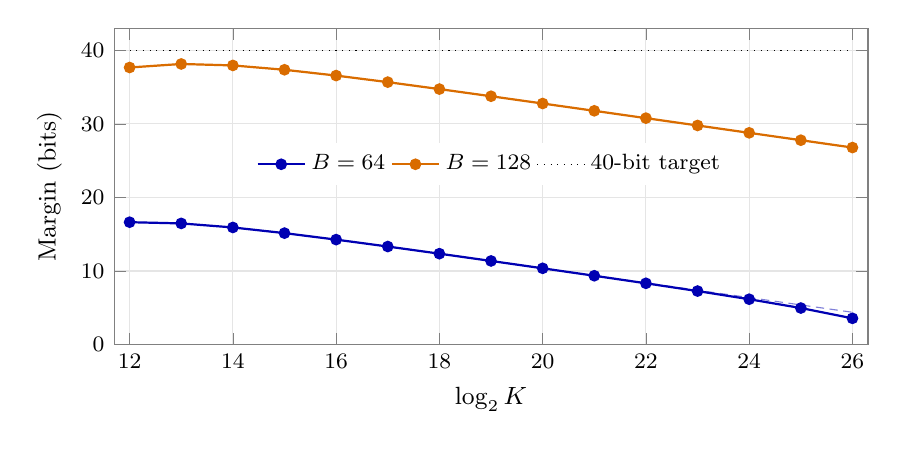
\begin{tikzpicture}
\begin{axis}[tick label style={font=\footnotesize},label style={font=\small},title style={font=\small},grid=major,grid style={black!10},axis line style={black!50},legend style={font=\footnotesize,draw=none},width=.92\linewidth,height=5.6cm,xlabel={$\log_2 K$},ylabel={Margin (bits)},xmin=11.7,xmax=26.3,ymin=0,ymax=43,xtick={12,14,16,18,20,22,24,26},ytick={0,10,20,30,40},legend style={at={(.5,.57)},anchor=center,legend columns=3},]
\addplot[blue!70!black,thick,mark=*,mark size=1.7pt,unbounded coords=jump] coordinates {(12,16.639117000) (13,16.473634000) (14,15.924509000) (15,15.153949000) (16,14.271217000) (17,13.331531000) (18,12.360479000) (19,11.371835000) (20,10.371924000) (21,9.361065000) (22,8.333885000) (23,7.278242000) (24,6.171264000) (25,4.972020000) (26,3.574425000)};
\addplot[blue!70!black,densely dashed,opacity=.5,unbounded coords=jump,forget plot] coordinates {(12,16.639437032) (13,16.473926576) (14,15.924885143) (15,15.154546125) (16,14.272276680) (17,13.333522500) (18,12.364337050) (19,11.379423850) (20,10.386947400) (21,9.390847400) (22,8.392758800) (23,7.393727000) (24,6.394199000) (25,5.394442000) (26,4.394563000)};
\addlegendentry{$B=64$}
\addplot[orange!85!black,thick,mark=*,mark size=1.7pt,unbounded coords=jump] coordinates {(12,37.661913000) (13,38.142752000) (14,37.943933000) (15,37.353947000) (16,36.564526000) (17,35.673924000) (18,34.729010000) (19,33.756062000) (20,32.769598000) (21,31.776503000) (22,30.780002000) (23,29.781637000) (24,28.782539000) (25,27.782972000) (26,26.783189000)};
\addplot[orange!85!black,densely dashed,opacity=.5,unbounded coords=jump,forget plot] coordinates {(12,37.661913061) (13,38.142752000) (14,37.943933000) (15,37.353947000) (16,36.564526000) (17,35.673924001) (18,34.729010002) (19,33.756062003) (20,32.769598006) (21,31.776503011) (22,30.780002023) (23,29.781637046) (24,28.782539091) (25,27.782972182) (26,26.783189364)};
\addlegendentry{$B=128$}
\addplot[black,dotted] coordinates {(12,40.000000000) (26,40.000000000)};
\addlegendentry{40-bit target}
\end{axis}
\end{tikzpicture}
\end{minipage}

\caption{Outer length and message length, with $(t,s)=(64,20)$ fixed.
Solid curves give full first-moment upper-bound margins; faint dashed curves
give the one-active-row ($q=1$) margins and mostly overlap the solid curves.
The inner map is shared across the two outer lengths. Points are evaluated
configurations; connecting segments are guides, not bounds between points.}
\label{fig:finite-k-b}
\end{figure}
